\chapter{Aspects énergétiques de l'électromagnétisme}

\section{Énergie Électromagnétique} % (fold)
\label{sec:Énergie Électromagnétique}

\subsection{Densité d'énergie électromagnétique} % (fold)
\label{sub:Densité d'énergie électromagnétique}

Pour établir un tel champ $\{ \overrightarrow{E}(M,t), \overrightarrow{B}(M,t)\}$ dans un petit volume d'espace au voisinage d'un point $M$, un opérateur doit \underline{fournir une énergie} : 
\begin{equation}
  \mathrm{d} W _{em}  = w _{em}(M,t) \mathrm{d}\tau_M
\end{equation}
% subsection Densité d'énergie électromagnétique (end)

avec $w _{em}$ est la \textbf{densité volumique d'énergie électromagnétique}, s'exprime en $\mathrm{J}. \mathrm{m} ^{-3}$, sous la forme (sans démonstration) : 
\begin{equation}
\boxed{ w _{em}(M,t) = \frac{1}{2}  \varepsilon_0 E ^{2}(M,t) + \frac{1}{2 \mu_0} B ^{2}(M,t)}
\end{equation}
% section ënergie Électromagnétique (end)

\subsection{Énergie électromagnétique} % (fold)
\label{sub:Énergie électromagnétique}

Dans un volume $V$ donné, l'énergie électromagnétique totale est la somme des énergies de chaque volume : 
\begin{equation}
  \boxed{ E _{em}(t) = \iiint _{(V)} w _{em}(M,t) \mathrm{d}\tau_M}
\end{equation}

Pour créér une distribution donné de charge il faut dépenser l'énergie électromagnétique associée qui règne dans tout l'espace.
% subsection Énergie électromagnétique (end)

\subsection{Situation statiques} % (fold)
\label{sub:Situation statiques}

\subsubsection{Condensateur plan} % (fold)
\label{sec:Condensateur plan}

\begin{figure}[H] %h:当前位置, t:顶部, b:底部, p:浮动页
  \centering
  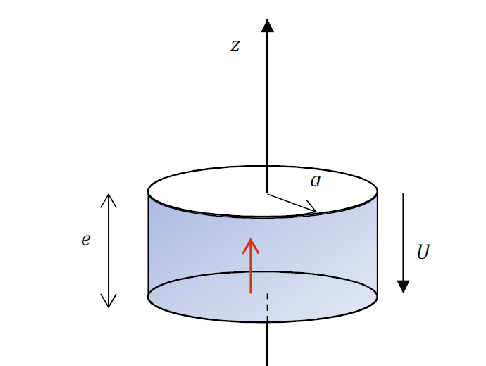
\includegraphics[width=0.4\textwidth]{./assets/Condensateur plan.png}
  \caption{Condensateur plan}
  \label{fig:Condensateur plan}
\end{figure}


Entre les armatures du condensateur : $\overrightarrow{E}= \frac{\sigma}{\varepsilon_0} \overrightarrow{e_z}$, ailleurs $\overrightarrow{E}= \overrightarrow{0}$. 
\begin{itemize}

    \item $Q = \sigma \pi a ^{2}$ 
    \item Énergie stockée : 
      \begin{align}
        W _{el} = E _{el} &= \iiint \frac{1}{2}  \varepsilon_0 E ^{2}\mathrm{d} \tau \\ 
                          &= \frac{1}{2}  \varepsilon_0 \frac{\sigma ^{2}}{\varepsilon_0 ^{2}} \pi a ^{2} e \\
                          &= \frac{1}{2}  \times \frac{\sigma ^{2} \pi a ^{2}}{\varepsilon_0} e \\
                          &= \frac{1}{2}  \frac{Q ^{2}}{C} 
     \end{align}

     \item Avec $C = \varepsilon_0 \frac{S}{l} $

\end{itemize}
% subsubsection Condensateur plan (end)

\subsubsection{Sphère chargée en surface} % (fold)
\label{sec:Sphère chargée en surface}


% subsubsection Sphère chargée en surface (end)

\subsubsection{Bobine parcourue par un courant} % (fold)
\label{sec:Bobine parcourue par un courant}

% subsubsection Bobine parcourue par un courant (end)
% subsection Situation statiques (end)

\newpage
\section{Transferts d'énergie électromagnétique} % (fold)
\label{sec:Transferts d'énergie électromagnétique}

\subsection{Révision: Puissance volumique locale fournie aux charges} % (fold)
\label{sub:Puissance volumique locale fournie aux charges}

Lorsque des \underline{charges} se déplacent dans un conducteur, la force électromagnétique fournit une certaine puissance : 
\begin{equation}
  \overrightarrow{F} _{\to q} = q ( \overrightarrow{E} + \overrightarrow{v} \wedge \overrightarrow{B})
\end{equation}

La puissance de cette force : 
\begin{equation}
  P _{\to q} = q (\overrightarrow{E} + \overrightarrow{v} \wedge \overrightarrow{B}). \overrightarrow{v} = q \overrightarrow{E}. \overrightarrow{v}
\end{equation}

Dans un petit volumne $\mathrm{d} \tau$ : 
\begin{equation}
  p_v = \frac{nq \times \mathrm{d}\tau \overrightarrow{E}. \overrightarrow{v}}{\mathrm{d}\tau}  = nq \overrightarrow{v}. \overrightarrow{E} = \overrightarrow{j}. \overrightarrow{E}
\end{equation}

Finalement, la \textbf{puissance volumique reçue par les charges} : 
\begin{equation}
  p_v (M) = \overrightarrow{j}(M). \overrightarrow{E}(M)
\end{equation}

% subsection Puissance volumique locale fournie aux charges (end)

\subsection{Vecteur de Poynting} % (fold)
\label{sub:Vecteur de Poynting}

On définit le \textbf{vecteur de Poynting}, ou \textbf{bilan local d'énergie électromagnétique} par : 
\begin{equation}
  \overrightarrow{\Pi}(M,t) = \frac{\overrightarrow{E}(M,t)\wedge \overrightarrow{B}(M,t)}{\mu_0} 
\end{equation}
s'exprime en $\mathrm{W}. \mathrm{m} ^{-2}$, il s'agit d'une \underline{puissance par unité de surface}.
% subsection Vecteur de Poynting (end)

\subsection{Équation locale de Poynting} % (fold)
\label{sub:Équation locale de Poynting}

L'\textbf{Équation locale de Poynting} s'écrit : 
\begin{equation}
  \boxed{ \mathrm{div}( \overrightarrow{\Pi(M,t)}) + \frac{\partial  w _{em}(M,t)}{\partial t} = - \overrightarrow{j}(M,t) . \overrightarrow{E}(M,t)}
\label{eq:Poynting}
\end{equation}
% subsection Équation locale de Poynting (end)

où 
\begin{equation}
  p_v (M,t) = \overrightarrow{j}(M,t). \overrightarrow{E}(M,t)
\end{equation}
représente la \textbf{puissance volumique locale fournie aux charges} par le biais de la force de Lorentz.

\begin{myproof}{}{}
\begin{itemize}

    \item Outil mathématique 1 : 
      \begin{equation}
        \mathrm{div} (\overrightarrow{E} \wedge \overrightarrow{E}) = \overrightarrow{B}. \overrightarrow{\mathrm{rot}} \overrightarrow{E} - \overrightarrow{E}. \overrightarrow{\mathrm{rot}}\overrightarrow{B}
      \end{equation} 

    \item Outil mathématique 2 : 
      \begin{equation}
        \frac{\partial }{\partial t} ( \overrightarrow{B}. \overrightarrow{B}) = 2 \overrightarrow{B}. \frac{\partial \overrightarrow{B}}{\partial t} 
      \end{equation}
    \item D'après l'équation Maxwell-Ampère : 
      \begin{gather}
        \overrightarrow{\mathrm{rot}} \overrightarrow{B} = \mu_0 \overrightarrow{j} + \varepsilon_0 \mu_0 \frac{\partial \overrightarrow{E}}{\partial t} \\ 
        \overrightarrow{j} = \frac{1}{\mu_0}  \overrightarrow{\mathrm{rot}} \overrightarrow{B} - \varepsilon_0 \frac{\partial  \overrightarrow{E}}{\partial t}
      \end{gather}

    En utilisant le résultat précédant : 
    \begin{align}
      \overrightarrow{j}. \overrightarrow{E} &= \frac{1}{\mu_0} [\overrightarrow{\mathrm{rot}}\overrightarrow{B}. \overrightarrow{E}] - \varepsilon_0 \frac{\partial \overrightarrow{E}}{\partial t} . \overrightarrow{E} \\ 
                                             &= \frac{1}{\mu_0} [\overrightarrow{B}. \overrightarrow{\mathrm{rot}} \overrightarrow{E} - \mathrm{div} ( \overrightarrow{E} \wedge \overrightarrow{B})] - \varepsilon_0 \frac{\partial \overrightarrow{E}}{\partial t} . \overrightarrow{E} \\ 
                                             &= \frac{1}{\mu_0} \left[ \overrightarrow{B}. \left( - \frac{\partial \overrightarrow{B}}{\partial t}  \right) - \mathrm{div} (\overrightarrow{E} \wedge \overrightarrow{B}) \right] - \varepsilon_0 \frac{\partial \overrightarrow{E}}{\partial t} . \overrightarrow{E} \\ 
                                             &= \frac{1}{\mu_0} \left[ \frac{1}{2} \frac{\partial }{\partial t} {B} ^{2} + \mathrm{div} (\overrightarrow{E} \wedge \overrightarrow{B}) \right] + \frac{\varepsilon_0}{2}  \frac{\partial E ^{2}                                            }{\partial t}
    \end{align}

\end{itemize}
\end{myproof}



\subsection{Bilan local dans le vide} % (fold)
\label{sub:Bilan local dans le vide}

Dans le vide, la densité de courant est nulle. Par conséquent, nous aurons : 
\begin{equation}
  \mathrm{div}(\overrightarrow{\Pi}(M,t)) + \frac{\partial w _{em}(M,t)}{\partial t}  = 0
\end{equation}

qui est à rapprocher de l'équation locale de conservation de la charge. 


% subsection Bilan local dans le vide (end)


\subsection{Bilan intégral d'énergie électromagnétique} % (fold)
\label{sub:Bilan intégral d'énergie électromagnétique}

Considérons une surface fermée délimitant un volume. L'énergie électromagnétique \underline{contenue dans ce volumne} est :
\begin{equation}
  E _{em}(t) = \iiint_{(V)} \mathrm{d} \tau_M
\end{equation}

Elle varie en fonction du temps, et d'après l'équation locale de Poynting \ref{eq:Poynting} : 
\begin{align}
  \frac{\mathrm{d}E _{em}}{\mathrm{d}t} (t) &= \iiint _{(V)} \frac{\partial w _{em}(M,t)}{\partial t} \mathrm{d} \tau_M \\ 
                                            &= \iiint _{(V)} - \mathrm{div} (\overrightarrow{\Pi}(M,t)) \mathrm{d} \tau_M - \iiint _{(V)} \overrightarrow{j}(M.t) . \overrightarrow{E}(M,t) \mathrm{d} \tau_M \\
                                            &= \iint _{(\Sigma)} \overrightarrow{\Pi}(M,t) . \overrightarrow{n} _{\text{int},M} \mathrm{d}S_M - P _{ \to \text{charges}}
\end{align}

Conclusion, l'énergie électromagnétique varie au cours du temps sous l'effet de deux causes : 
\begin{itemize}

    \item l'énergie qui est \underline{donnée aux charges}
    \item terme complémentaire s'exprime comme un flux à travers la surface limitant le volume $(V)$

\end{itemize}


% subsection Bilan intégral d'énergie électromagnétique (end)

% subsection Bilan intégral (end)

% subsection Bilan in'tegral (end)
% section Transferts d'énergie électromagnétique (end)

\newpage
\section{Exemples} % (fold)
\label{sec:Exemples}

\subsection{Solénoïde parcouru par un courant variable} % (fold)
\label{sub:Solénoïde parcouru par un courant variable}

\begin{figure}[H] %h:当前位置, t:顶部, b:底部, p:浮动页
  \centering
  \includegraphics[width=0.8\textwidth]{./assets/Solénoïde parcouru par un courant variable.png}
  \caption{Solénoïde parcouru par un courant variable}
  \label{fig:Solénoïde parcouru par un courant variable}
\end{figure}


\begin{itemize}

    \item  Symétrie et invariance : $\overrightarrow{E}(M,t) = E(r,t) \overrightarrow{e_ \theta}$, $\overrightarrow{B}(M,t) = B(r,t) \overrightarrow{e_z}$ 

    \item Dans l'ARQS, $\overrightarrow{B}(M,t) = \overrightarrow{B} _{QS}(M,t) = \mu_0 n I \overrightarrow{e_z}$ à l'intérieur et $\overrightarrow{0}$ à l'extérieur.

    \item À l'aide de la loi de Faraday, on obtient 
      \begin{equation}
        E(r,t) = \begin{cases}
          - \mu_0 \frac{nr}{2}  \frac{\mathrm{d}I(t)}{\mathrm{d}t}  \quad (r<R) \\ 
          - \mu_0 n \frac{R ^{2}}{2r}  \frac{\mathrm{d}I(t)}{\mathrm{d}t}  \quad (r>R)
        \end{cases}
      \end{equation}

      \begin{tcolorbox}
          On observe que à l'extérieur du solénoïde, $\overrightarrow{B}(M,t) = \overrightarrow{0}$ alors que $\overrightarrow{E}(M,t) \ne \overrightarrow{0}$. Comme $\overrightarrow{E}$ selon $\overrightarrow{e_ \theta}$, les lignes de champ sont fermées (différent du cas d'électrostatique)
      \end{tcolorbox}

    \item À l'intérieur, La densité d'énergie dans le solénoïde est essentiellement sous forme \underline{magnétique}
      \begin{myproof}{}{}
      On les exprime : 
      \begin{equation}
        w _{el} = \frac{1}{2}  \varepsilon_0 \left( - \mu_0 n \frac{r}{2} \frac{\mathrm{d}I}{\mathrm{d}t} \right) ^{2}, \quad w _{mag} = \frac{1}{2 \mu_0}  (\mu_0 n I(t)) ^{2}
      \end{equation}

      La proportion : 
      \begin{equation}
        \frac{w _{mag}}{w _{el}} = \frac{1}{\mu_0 \varepsilon_0}  \frac{4}{r ^{2}}  \frac{I ^{2}(t)}{ \left( \frac{\mathrm{d}I}{\mathrm{d}t}  \right) ^{2}       } 
      \end{equation}

      Pour un courant variable du type $I(t) = I_0 \cos \omega t$, $\langle I ^{2} \rangle = I_0 ^{2}/ 2$ et $\langle \dot{I}^{2}\rangle = I_0 ^{2} \omega ^{2}/2$ : (Rappel : $\mu_0 \varepsilon_0 c ^{2} = 1$)
      \begin{equation}
        \frac{ \langle w _{mag} \rangle}{ \langle w _{el} \rangle} = \frac{4 c ^{2}}{r ^{2} \omega ^{2}} 
      \end{equation}

      La condition d'\textbf{ARQS} s'impose : $R \ll \lambda$ donc $r \ll c \times 2 \pi /\omega$. 
      Enfin, 
      \begin{equation}
        \frac{ \langle w _{mag} \rangle}{ \langle w _{el} \rangle}  \gg \frac{1}{\pi ^{2}} 
      \end{equation}
      \end{myproof} 

    \item Le vecteur de Poynting : 
      \begin{equation}
        \overrightarrow{\Pi}(t) =  \frac{\overrightarrow{E} \wedge \overrightarrow{B}}{\mu_0}  = - \mu_0 n ^{2} \frac{r}{2}  I(r) \frac{\mathrm{d}I(t)}{\mathrm{d}t}  \overrightarrow{e_r}
      \end{equation}

    \item Puissance électromagnétique rentrante : 
      \begin{equation}
        - \iint _{(S)} \overrightarrow{\Pi}(r= R ^{-}, t) . \mathrm{d} \overrightarrow{S}_{ext} = + \mu_0 n ^{2} R I(t) \frac{\mathrm{d}I(t)}{\mathrm{d}t}  \pi R l
      \end{equation}
    \item Cas $r = R ^{-}$. Variation d'énergie électromagnétique dans le volume vide $(V)$ : 
      \begin{align}
        \frac{\mathrm{d} w _{em}}{ \mathrm{d}t}  &= \mu_0 n ^{2} R ^{2} \pi l \frac{\mathrm{d}}{\mathrm{d}t}  \left( \frac{1}{2}  I ^{2}(t) \right) \\ 
                                                 &= \frac{\mathrm{d}}{\mathrm{d}t}  \left( \frac{1}{2} LI ^{2}(t))
                                                 \right) \text{ avec } L = \mu_0 n ^{2} R ^{2} \pi l = \mu_0 \frac{N ^{2}}{l}  R ^{2} \pi
      \end{align}

    \item Cas $r = R ^{+}$. Comme $\overrightarrow{B} _{ext} = \overrightarrow{0}$ donc $\overrightarrow{\pi}(r = R ^{+}, t) = \overrightarrow{0}$. 
      \begin{equation}
        \frac{\mathrm{d} W _{em}}{\mathrm{d} t}  = - \iiint _{(V)} \overrightarrow{j}(M,t) \overrightarrow{E}(M,t) \mathrm{d} \tau
      \end{equation}

      Par continuité : 
      \begin{equation}
        \frac{\mathrm{d}W _{em}}{  \mathrm{d} t} | _{r = R ^{-}} = 
        \frac{\mathrm{d}W _{em}}{  \mathrm{d} t} | _{r = R ^{+}}
      \end{equation}

      Résultat : L'énergie électromagnétique du système est intégralement prélevée ou fournie aux \underline{charges} qui circulent dans le solénoïde : 
      \begin{equation}
        P _{\to q} = - \frac{\mathrm{d}}{\mathrm{d}t}  \left( \frac{1}{2}  L I ^{2} \right)
      \end{equation}
      




      

\end{itemize}

% subsection Solénoïde parcouru par un courant variable (end)

\subsection{Condensateur plan circulaire} % (fold)
\label{sub:Condensateur plan circulaire}

% subsection Condensateur plan circulaire (end)
\subsection{Résistance} % (fold)
\label{sub:Résistance}

% subsection Résistance (end)

% section Exemples (end)
% chapter Énergie électromagnétisme (end)
